\documentclass[tikz]{standalone}
\usepackage{tikz}
\usepackage{alphalph}
\usetikzlibrary{positioning, graphs}
\usetikzlibrary{graphs.standard}
\begin{document}
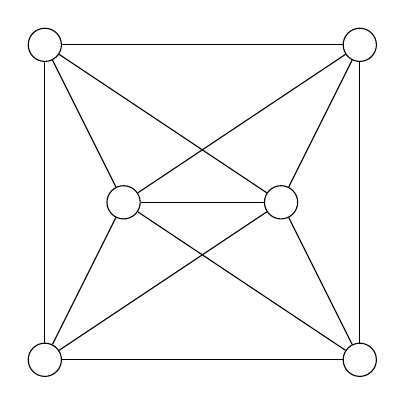
\begin{tikzpicture}
\begin{scope}
		[vertex/.style={draw,circle,inner sep = 0em, minimum size = 1.2em},
		 edgelabel/.style = {fill = white, inner sep = 0.2em, font=\small}]
		\node[vertex] (a) at (0, 0) {};
		\node[vertex] (b) at (4, 0) {};
		\node[vertex] (c) at (1, 2) {};
		\node[vertex] (d) at (3,2) {};
		\node[vertex] (e) at (0,4) {};
		\node[vertex] (f) at (4,4) {};
		
		\draw[-] (a) -- (b);
		\draw[-] (a) -- (c);
		\draw[-] (a) -- (d);
		\draw[-] (a) -- (e);
		\draw[-] (b) -- (c);
		\draw[-] (b) -- (d);
		\draw[-] (b) -- (f);
		\draw[-] (c) -- (d);
		\draw[-] (c) -- (e);
		\draw[-] (c) -- (f);
		\draw[-] (d) -- (e);
		\draw[-] (d) -- (f);
		\draw[-] (e) -- (f);
		
\end{scope}
\end{tikzpicture}
\end{document}